% Beginning of a chapter
% Use labels for referencing
\chapter{Entrancess}\label{entrances} 
\section{Introduction}\label{intro}
% this is a comment
% normal text
This section will describe the process of 

Also we wanted to know more about how people enter a building. Since the location of most aps is known for BK, this is our case study. This is an interesting and challenging use case at the same time. BK is a building having multiple entrances; 5, main, west, east and two south (modelling hall). Knowing what entrances are used, when what entrances are used and how frequent they are used, will give insight into the use of a building, the spatial context and the relation between these two. It bridges the gap between the spatial levels. For this we will make use of  
\\
How do we want to find answers? Be looking at the first and last connection with an ap in a stay. 

wekjfdhwekfhw \\

\section{Hypothesis}\label{hypo}
Our hypothesis is that finding clear answers to the questions is going to be hard. Firstly, because the existing ap layout is not designed for this purpose and therefore there are not always aps located near an entrance. Secondly, because the logging frequency is just a little more than 5 min. Ideally we would like the device to get scanned first at the very first ap it connects with. But because  of the logging frequency you have to be lucky. You have to connect with the ap near the entrance exactly at the time it logs the connected devices. 
\\
But still we expect to see some results. The ap near the main entrance, assuming this entrance is used by most people, would still...





Begin numbered list
\begin{enumerate}
\item number 1
\item number 2
\item number 3
\item number 4
\end{enumerate}
Begin bullet list
\begin{itemize}
\item this is a bullet
\item this as well
\end{itemize}


\section{Include graphics}
To include graphics in the document, use the following template:

\begin{figure}[H]
\centering
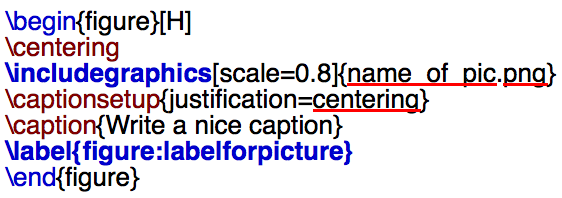
\includegraphics[scale=0.8]{name_of_pic.png}
\captionsetup{justification=centering}
\caption{Write a nice caption}
\label{figure:labelforpicture}
\end{figure}

If you want to refer to a picture (or section/chapter/whatever) in the text, this can be done using the 'autoref' function. \autoref{figure:labelforpicture} shows how to include graphics in a document. This also works for sections: \autoref{movementpatterns}.

\section{Tables}
Use \url{http://www.tablesgenerator.com} for creating nice looking tables. Use the 'booktabs' style!!!
\begin{table}[H]
\centering
\caption{My caption}
\label{my-label}
<<<<<<< HEAD
\begin{tabular}{lll}[H]
\hline
this & is      & a      \\ \hline
=======
\begin{tabular}{@{}lll@{}}
\toprule
this & is      & a      \\ \midrule
>>>>>>> 3dc9814e185ffebcba50bc64c0886fdaf49dc3d0
nice & looking & table  \\
am   & i       & right? \\ \bottomrule
\end{tabular}
\end{table}
Unfortunately, LaTeX always places tables at the top or bottom of a page, so it will mostly mess up the layout! Use proper referencing in the text to make sure tables are read as they should! \autoref{my-label}.

\section{Referencing}
It would be nice if everyone could go over the parts they have written in the mid-term review and find everything they have referenced. You can easily import biblatex styled references from google scholar. If you search in google scholar for a title, there is usually a link below the result, 'cite'. Then you can select 'bibtex' as an option to download a file. The text inside this file can be copied into the 'report.bib' file. If you want to cite an author, that can be done using the 'cite' option. i.e. this author was used in the mid term review:
Let's cite! The Einstein's journal paper \cite{mautz2012indoor} and the Dirac's 
book \cite{meneses2012large} are physics related items. 

\section{bold and italics}
\textbf{this text will be bold!}
\textit{this text will be in italics}




